% !TeX root = ..\main.tex
\section{Lược đồ BPMN}
\subsection{Tổng quan về BPMN}
\hspace*{0.5cm}BPMN(Business Process Modeling Notation) là một lược đồ tập hợp các kí hiệu để mô hình hóa trực quan các quy trình nghiệp vụ xử lý . BPMN giúp các doanh nghiệp trực quan hóa các hoạt động và các luồng thông tin để thực hiện quy trình nghiệp vụ.
\begin{figure}[!htp]
    \centering
    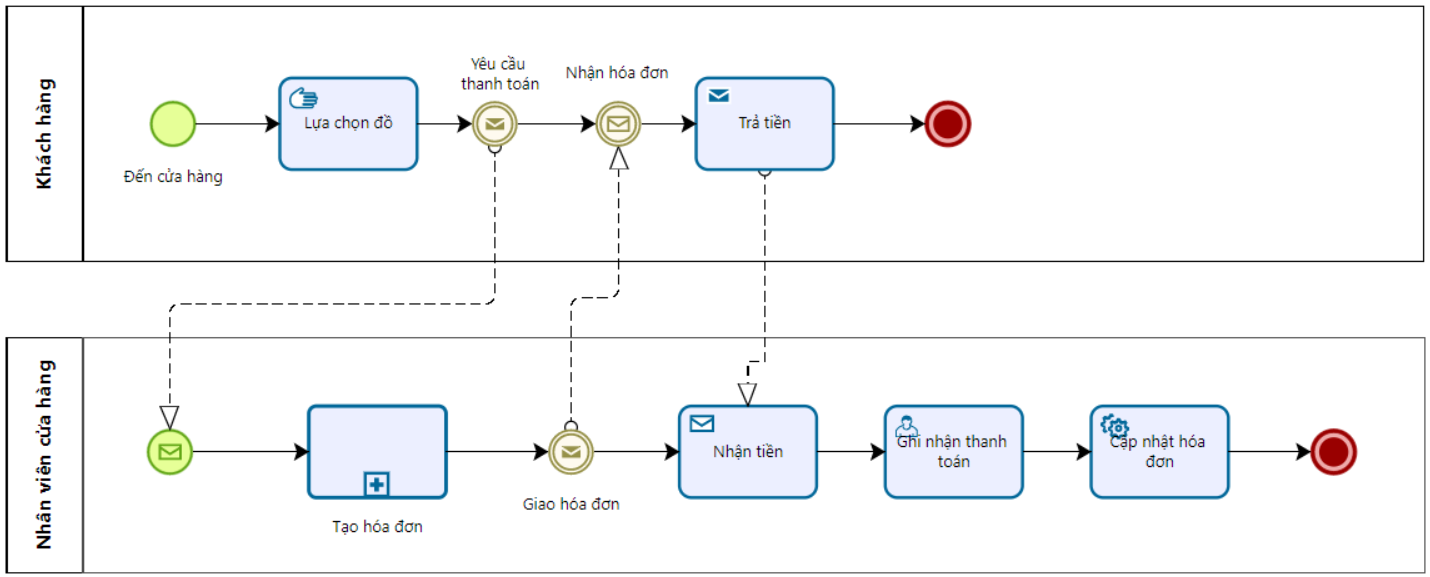
\includegraphics[width=10cm]{img/theory/BPMN/BPMN_sample.png}
    \newline
    \caption{Ví dụ về lược đồ BPMN}
\end{figure}
 
 
 
\subsection{Lợi ích của BPMN}
\begin{itemize}
    \item Giúp các bên liên quan có thể hiểu rõ quy trình nghiệp vụ của hệ thống
    \item Thu hẹp khoảng cách giữa bộ phận thiết kế và bộ phận nghiệp vụ
    \item Dễ dàng mô tả các nghiệp vụ phức tạp
\end{itemize}
 
\subsection{Các thành phần của BPMN}
\subsubsubsection*{Swimlane}
Swimlane bao gồm Pool và Lane:
\begin{itemize}
    \item Pool: Đại diện cho một tổ chức, phòng ban, một vai trò hoặc một hệ thống nào đó.
    \item Lane: Đại diện các cá nhân riêng lẻ, người sẽ làm các hoạt động cụ thể.
\end{itemize}
\newpage
\begin{figure}[!htp]
    \centering
    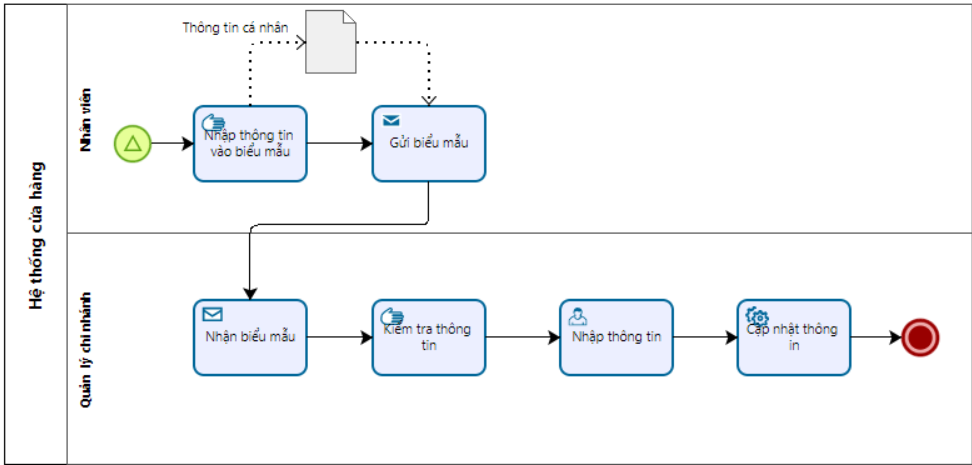
\includegraphics[width=10cm]{img/theory/BPMN/BPMN_swimlane.png}
    \newline
    \caption{Lược đồ BPMN bao gồm 1 pool(Hệ thống cửa hàng) và 2 lane (Nhân viên, Quản lý chi nhánh)}
\end{figure}
\subsubsubsection*{Activities}
Mô tả công việc trong quy trình, được kí hiệu bằng một hình chữ nhật bo tròn 4 góc, bao gồm 4 loại:
\begin{itemize}
    \item Task: Các việc nhỏ, đơn lẻ
          \begin{figure}[!htp]
              \begin{center}
                  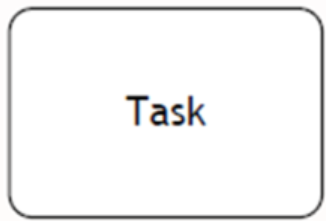
\includegraphics[width=2cm]{img/theory/BPMN/Task.png}
              \end{center}
              \caption{Task \cite{theoryBPMN0}}
          \end{figure}
    \item Event Sub-Process: Một quy trình con nằm trong một quy trình lớn, chức nhiều task
          \begin{figure}[!htp]
              \begin{center}
                  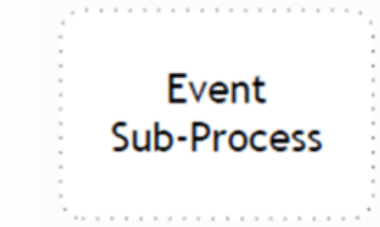
\includegraphics[width=2cm]{img/theory/BPMN/Event Sub-process.png}
              \end{center}
              \caption{Event Sub-Process \cite{theoryBPMN0}}
          \end{figure}
    \item Transaction: Các giao dịch, bao gồm các task nhỏ khác logic với nhau
          \begin{figure}[!htp]
              \begin{center}
                  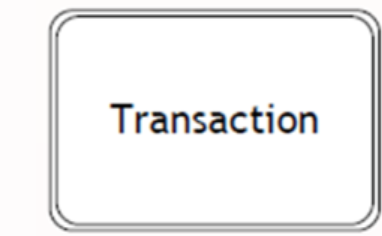
\includegraphics[width=2cm]{img/theory/BPMN/Transaction.png}
              \end{center}
              \caption{Transaction \cite{theoryBPMN0}}
          \end{figure}
    \item Call Activity: Gọi một quy trình khác đã được định nghĩa trong hệ thống, thay vì phải định nghĩa lại nhiều lần
          \begin{figure}[!htp]
 
              \begin{center}
                  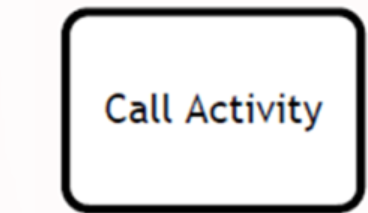
\includegraphics[width=2cm]{img/theory/BPMN/Call Activity.png}
              \end{center}
              \caption{Call Activity \cite{theoryBPMN0}}
          \end{figure}
\end{itemize}


\subsubsubsection*{Events}
Sự kiện là một tác động đến quy trình nghiệp vụ có thể là bên ngoài hoặc bên trong. Các sự kiện thường được kí hiệu bằng hình tròn, bên trong có các kí hiệu về loại hình kích hoạt. Bao gồm các loại:
\begin{itemize}
	\item Start: Các sự kiện mở đầu quy trình nghiệp vụ
	\item Intermediate: Các sự kiện xảy ra giữa các quy trình nghiệp vụ
	\item End: Các sự kiện kết thúc quy trình nghiệp vụ
\end{itemize}
\begin{figure}[!htp]
	\begin{center}
		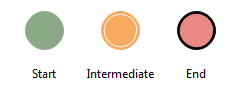
\includegraphics[width=6cm]{img/theory/BPMN/Event.png}
	\end{center}
	\caption{Các loại sự kiện trong BPMN \cite{theoryBPMN1}}
\end{figure}


\subsubsubsection*{Gateways}
Các cổng có nhiệm vụ chính là kiểm soát dòng chảy của quy trình nghiệp vụ. Cổng thường kí hiệu hình thoi, bên trong là ký hiệu các loại.
\begin{itemize}
    \item Start: Các sự kiện mở đầu quy trình nghiệp vụ
    \item Intermediate: Các sự kiện xảy ra giữa các quy trình nghiệp vụ
    \item End: Các sự kiện kết thúc quy trình nghiệp vụ
\end{itemize}
\begin{figure}[!htp]
    \begin{center}
        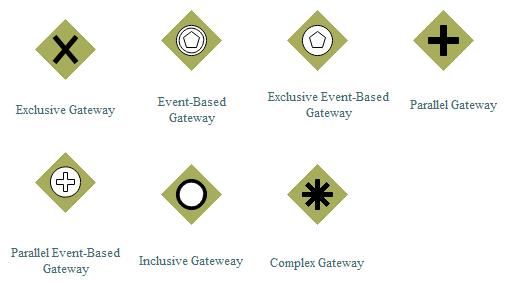
\includegraphics[width=8cm]{img/theory/BPMN/Gateway.png}
    \end{center}
    \caption{Các loại cổng phổ biến trong BPMN \cite{theoryBPMN1}}
\end{figure}



%%%%%%%%%%%%%%%%%%%%%%%%%%%%%%%%%
\section{Ngôn ngữ BPEL}
\subsection{Tổng quan về BPEL}
\hspace*{0.5cm} BPEL hay BPEL4WS(Business Process Execution Language for Web Services) là ngôn ngữ dùng để định nghĩa và thực thi các quy trình nghiệp vụ sử dụng các dịch vụ web. Ngôn ngữ BPEL được xây dựng dựa trên nền tảng XML hỗ trợ các dịch vụ web: SOAP, WSDL, UDDI. BPEL xây dựng một dịch vụ web dựa trên việc điều phối, phối hợp các dịch vụ web độc lập khác để hình thành nên một dịch vụ web mới.
\subsection{Các thành phần trong BPEL}
BPEL bao gồm các thành phần nguyên tố và các thành phần cấu trúc. Các thành phần nguyên tố bao gồm:
\begin{itemize}
	\item $<invoke>$: Gọi một dịch vụ web khác
	\item $<receive>$: Đợi phản hồi tự các tác vụ bất đồng bộ
	\item $<reply>$: Phản hồi cho các tác vụ đồng bộ
	\item $<assign>$: Gán giá trị cho biến
	\item $<throw>$: Chỉ định các lỗi, ngoại lệ
	\item $<wait>$: Đợi một thời gian
	\item $<terminate>$: Kết thúc toàn bộ quy trình
\end{itemize}

Bên cạnh thành nguyên tố, các thành phần cấu trúc chứa nhiều tác vụ bên trong:
\begin{itemize}
    \item $<sequence>$: Các tác vụ thực hiện tuần tự
    \item $<flow>$: Các tác vụ thực hiện song song
    \item $<switch>$: Thực hiện các tác vụ rẽ nhánh
    \item $<while>$: Thực hiện các vòng lặp
\end{itemize}
 
Ngoài ra, còn có $<partnerLink>$ dùng để xác định các đối tác, các dịch vụ web sử dụng, $<variable>$ để định nghĩa các biến cần thiết trong quy trình


\subsection{Ví dụ về BPEL}
 
\hspace*{0.5cm} Để hiểu rõ về quy trình được mô tả bằng BPEL, ta xem xét ví dụ về quy trình sắp xếp chuyến đi cho nhân viên \cite{theoryBPEL}. Đầu tiên, chúng ta sẽ kiểm tra hạng vé của nhân viên, giả sử rằng có một dịch vụ web Employee Travel sẽ làm việc này. Sau đó, chúng ta kiểm tra giá vé của hai hãng: American Airlines và Delta Airlines để chọn ra giá vé thấp hơn và trả lại kết quả. Quy trình này được minh họa như sau:
 
\begin{figure}[!htp]
    \begin{center}
        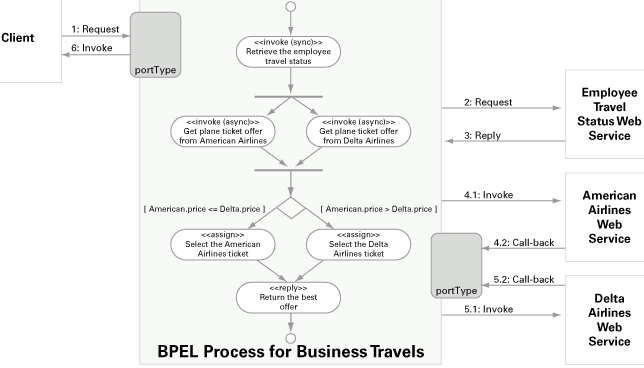
\includegraphics[width=10cm]{img/theory/BPEL/Sample.png}
    \end{center}
    \caption{Ví dụ về quy trình BPEL sắp xếp chuyến đi \cite{theoryBPEL}}
\end{figure}

Trong ví dụ này, các partner của hệ thống sẽ bao gồm Client, Employee Travel Status Web Service, American Airlines Web Service, Delta Airlines Web Service. Chúng ta sẽ xây dựng một quy trình BPEL bất đồng bộ, giả định rằng dịch vụ web Employee Travel là đồng bộ vì dữ liệu nhân viên đã có sẵn trong hệ thống chúng ta.
 
Quy trình BPEL chi tiết như sau: Đầu tiên Client sẽ gửi một yêu cầu bất đồng bộ kèm theo thông tin chuyến đi đến hệ thống. Hệ thống sẽ nhận thông tin và thực hiện lệnh gọi đồng bộ sang dịch vụ web Employee Travel để lấy thông tin hạng vé của nhân viên này. Tiếp theo, hệ thống sẽ thực hiện 2 lệnh gọi bất đồng bộ đồng thời đến 2 dịch vụ web của American Airlines và Delta Airlines để xác định giá vé. Sau khi hệ thống nhận được phản hồi kết quả của 2 hãng hàng không, hệ thống thực hiện so sánh để tìm giá vé thấp hơn và trả lại kết quả cho Client.

\subsection{Các bước xây dựng quy trình BPEL}
Để xây dựng ví dụ trên, ta cần thực hiện các bước sau:
\begin{enumerate}
	\item Xác định các dịch vụ web liên quan: Xác định các dịch vụ web tương tác đối với hệ thống (Employee Travel Web Service, American Airlines Web Service, Delta Airlines Web Service)
	\item Xây dựng WSDL cho quy trình BPEL: BPEL là một dịch vụ web, do đó ta cần xây dựng WSDL cho chính nó
	\item Xác định partnerLink cho quy trình: Cần xác định các dịch vụ web được thực hiện đồng bộ hay bất đồng bộ, cần những tham số nào để gọi.
	\item Xây dựng quy trình: Xây dựng các luồng đi, logic trong quy trình
\end{enumerate} 


%%%%%%%%%%%%%%%%%%%%%%%%%%%%%%%%%

\section{Chuyển đổi BPMN sang BPEL}
\hspace*{0.5cm} \par Việc chuyển đổi từ BPMN sang BPEL sẽ giúp tự động hóa quy trình nghiệp vụ. BPMN ở dạng diagram, là mô hình và công cụ để người dùng nghiệp vụ và lập trình viên có thể làm việc và giao tiếp với nhau. 
Còn để thực thi được nghiệp vụ, chúng ta cần ngôn ngữ thực thi, ở đây là BPEL. Vậy nên việc chuyển đổi từ BPMN sang BPEL là bước quan trọng trong việc tự động hóa quy trình nghiệp vụ.

\par Đầu tiên, ta đề cập đến các cấu trúc well-structured trong BPMN. Đây là các cấu trúc cơ bản, và dễ dàng để convert sang BPEL, do đó đây sẽ là nền tảng trong việc chuyển đổi. Các cấu trúc well-structured bao gồm:
\begin{itemize}
	\item Sequence
	\item Flow
	\item Switch
	\item Pick
	\item While
	\item Repeat
	\item Repeat - While
\end{itemize}

\par Với các cấu trúc phức tạp hơn, ta gọi các cấu trúc đó là non-well structured. Đối với cấu trúc này, ta có thể chia nhỏ và gom nhóm các thành phần của cấu trúc để tạo nên các well-structured, và từ đó chuyển đổi từng phần well-structured nhỏ sang BPEL. 
Sau đó ta gộp các thành phần BPEL đã chuyển đổi để thành BPEL cuối cùng.

\par Giải thuật chuyển đổi từ BPMN X sang BPEL như sau \cite{theoryConvert}:
\begin{enumerate}
	\item Nếu X là well-structured, chuyển đổi trực tiếp sang BPEL, tới bước 4.
	\item Nếu X là non-well structured:
	\begin{enumerate}
		\item Nếu tồn tại thành phần C là Sequence, chọn ra phần đó và đến bước 2.4.
		\item Nếu tồn tại thành phần C là well-structured và non-sequence, chọn ra phần đó và đến bước 2.4.
		\item Nếu tồn tại thành phần C là non-well structured, chọn ra phần đó.
		\item Gán việc ánh xạ C qua BPEL cho công việc t\_{c}.
		\item Quay lại bước 2.
	\end{enumerate}
	\item Xuất ra đoạn code ứng với công việc t\_{c}.
	\item Event nhập và event xuất được ánh xạ tương ứng lần lượt thành <process> và </process> để bao lại phần code BPEL vừa được chuyển đổi.
\end{enumerate}